\documentclass[aspectratio=169,11pt]{beamer}
\usepackage[T1]{fontenc}
\usepackage{lmodern,amsmath,amssymb,mathtools,bm,booktabs,array,graphicx,tikz}
\usetikzlibrary{arrows.meta,positioning,calc,decorations.pathreplacing,patterns}
\definecolor{ink}{HTML}{17344D}\definecolor{accent}{HTML}{087E8B}\definecolor{pale}{HTML}{EDF5F5}\definecolor{gold}{HTML}{AD6B19}
\providecommand{\dd}{\,\mathrm{d}}\providecommand{\R}{\mathbb{R}}
\providecommand{\E}{\mathbb{E}}\providecommand{\Var}{\operatorname{Var}}
\providecommand{\Cov}{\operatorname{Cov}}\providecommand{\diag}{\operatorname{diag}}
\providecommand{\norm}[1]{\left\lVert#1\right\rVert}
\providecommand{\abs}[1]{\left|#1\right|}
\usefonttheme{professionalfonts}
\setbeamercolor{normal text}{fg=black,bg=white}
\setbeamercolor{frametitle}{fg=ink,bg=white}
\setbeamercolor{title}{fg=ink}\setbeamercolor{structure}{fg=accent}
\setbeamercolor{block title}{fg=ink,bg=pale}\setbeamercolor{block body}{fg=black,bg=pale!40}
\setbeamercolor{alerted text}{fg=accent}
\setbeamerfont{frametitle}{size=\Large,series=\bfseries}
\setbeamerfont{title}{size=\LARGE,series=\bfseries}
\setbeamertemplate{navigation symbols}{}
\setbeamersize{text margin left=.7cm,text margin right=.7cm}
\setbeamertemplate{frametitle}{\vspace{.18cm}\insertframetitle\par\vspace{.1cm}{\color{accent}\hrule height .6pt}\vspace{.12cm}}
\newcommand{\notestarget}{notes.pdf}\newcommand{\noteslabel}{Notes}
\setbeamertemplate{footline}{\hspace{.7cm}\color{ink}\scriptsize Scientific Computing in Python\quad\href{\notestarget}{\noteslabel}\hfill\insertframenumber\,/\,\inserttotalframenumber\hspace{.7cm}\vspace{.18cm}}
\setbeamercovered{invisible}
\hypersetup{pdfauthor={Zan Ahmad},pdftitle={Functions, control flow, and threshold statistics},pdfpagemode=UseNone}
\begin{document}
\begin{frame}[plain]\vfill
{\small\color{accent} Scientific Computing in Python \quad Lecture 2}\par\medskip
{\raggedright\hyphenpenalty=10000\exhyphenpenalty=10000\LARGE\bfseries\color{ink} Functions, control flow, and threshold statistics}\par\bigskip
Zan Ahmad\par\smallskip
{\small Winter 2026}\par\vfill\end{frame}
\renewcommand{\notestarget}{notes.pdf\#note-a-three-valued-classification-rule}
\begin{frame}[t,fragile,label=slide-a-three-valued-classification-rule]{A three-valued classification rule}
\[
c(x;\theta)=\begin{cases}\text{missing},&x\text{ absent},\\\text{at or below},&x\leq\theta,\\\text{above},&x>\theta.\end{cases}
\]
\pause{}
At $\theta=40$, the values $40$ and $40.1$ belong to different classes.
\end{frame}
\renewcommand{\notestarget}{notes.pdf\#note-a-three-valued-classification-rule}
\begin{frame}[t,fragile,label=slide-a-function-implementing-the-partition]{A function implementing the partition}
\begin{verbatim}
def classify(value, target):
    if value is None:
        return "missing"
    if value <= target:
        return "at_or_below"
    return "above"
\end{verbatim}
\end{frame}
\renewcommand{\notestarget}{notes.pdf\#note-arguments-returns-and-local-names}
\begin{frame}[t,fragile,label=slide-arguments-returns-and-local-names]{Arguments, returns, and local names}
\begin{verbatim}
category = classify(35, 40)
print(category)
\end{verbatim}
\pause{}
The returned string is a value. The function can be called again with a different threshold without changing its definition.
\end{frame}
\renewcommand{\notestarget}{notes.pdf\#note-a-three-valued-classification-rule}
\begin{frame}[t,fragile,label=slide-boundary-cases]{Boundary cases}
\begin{center}\begin{tabular}{lll}\toprule
Reading & Threshold & Category\\\midrule
\texttt{None}&40&missing\\40&40&at or below\\40.1&40&above\\\bottomrule\end{tabular}\end{center}
\pause{}
Testing the boundary establishes whether the implemented inequality agrees with the definition.
\end{frame}
\renewcommand{\notestarget}{notes.pdf\#note-indicators-and-accumulated-counts}
\begin{frame}[t,fragile,label=slide-indicators-and-accumulated-counts]{Indicators and accumulated counts}
\[
N_{\leq}(\theta)=\sum_{i:\,x_i\text{ known}}\mathbf1_{\{x_i\leq\theta\}}.
\]
\pause{}
After $k$ observations,
\[
N_{\leq}^{(k)}+N_{>}^{(k)}+N_{\rm missing}^{(k)}=k.
\]
\end{frame}
\renewcommand{\notestarget}{notes.pdf\#note-the-first-recorded-qualifying-time}
\begin{frame}[label=slide-recorded-threshold-attainment-figure]{Recorded threshold attainment}
\centering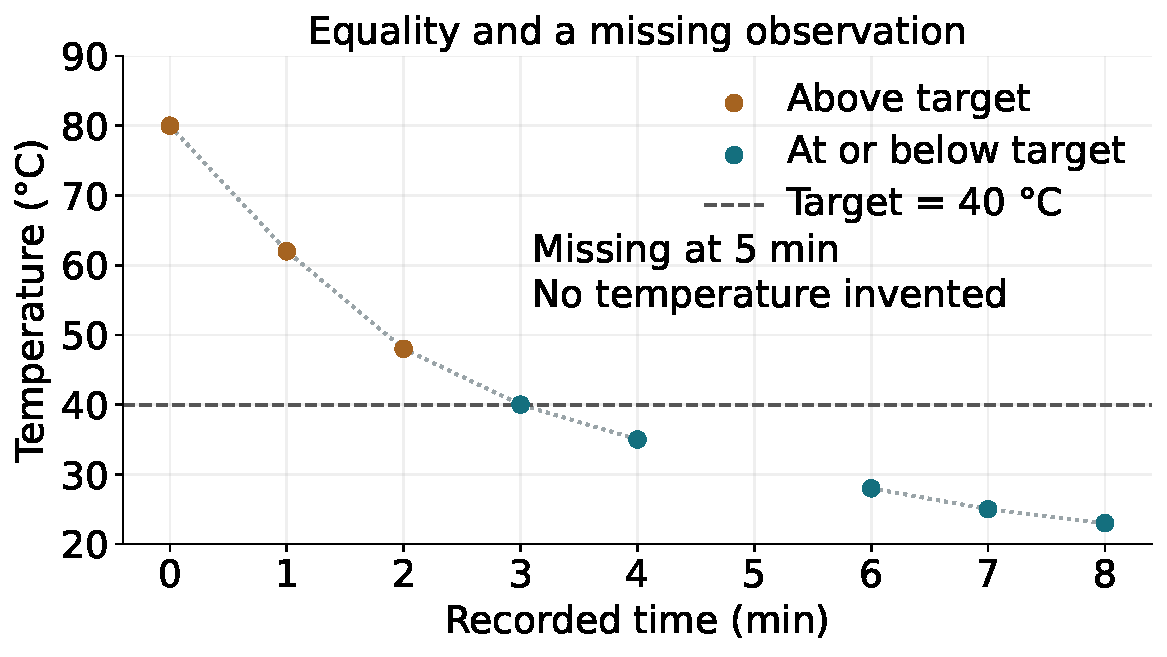
\includegraphics[width=.98\linewidth,height=.69\textheight,keepaspectratio]{presentation-figures/threshold-record.pdf}\end{frame}
\renewcommand{\notestarget}{notes.pdf\#note-indicators-and-accumulated-counts}
\begin{frame}[t,fragile,label=slide-the-nine-reading-example]{The nine-reading example}
\[
80,62,48,40,35,\text{missing},28,25,23.
\]
At threshold $40$:
\pause{}
\[
N_{\leq}=5,\quad N_>=3,\quad N_{\rm missing}=1.
\]
The counter identity gives $5+3+1=9$.
\end{frame}
\renewcommand{\notestarget}{notes.pdf\#note-the-denominator-of-a-proportion}
\begin{frame}[t,fragile,label=slide-the-denominator-of-a-proportion]{The denominator of a proportion}
\[
f(\theta)=\frac{N_{\leq}(\theta)}{N_{\rm known}},\qquad N_{\rm known}>0.
\]
\pause{}
For the supplied record,
\[
f(40)=\frac58=0.625.
\]
\end{frame}
\renewcommand{\notestarget}{notes.pdf\#note-monotonicity-of-threshold-counts}
\begin{frame}[t,fragile,label=slide-changing-the-threshold]{Changing the threshold}
At threshold $35$, only $35,28,25,23$ qualify:
\[
f(35)=\frac48=0.5.
\]
\pause{}
The known-reading denominator remains $8$ because the data and missingness did not change.
\end{frame}
\renewcommand{\notestarget}{notes.pdf\#note-the-first-recorded-qualifying-time}
\begin{frame}[t,fragile,label=slide-the-first-recorded-qualifying-time]{The first recorded qualifying time}
\[
t_{\rm first}=\min\{t_i:x_i\text{ known and }x_i\leq\theta\}.
\]
\pause{}
For observations at integer minutes and $\theta=40$, $t_{\rm first}=3$ min.
\end{frame}
\renewcommand{\notestarget}{notes.pdf\#note-monotonicity-of-threshold-counts}
\begin{frame}[label=slide-threshold-count-as-a-step-function-figure]{Threshold count as a step function}
\centering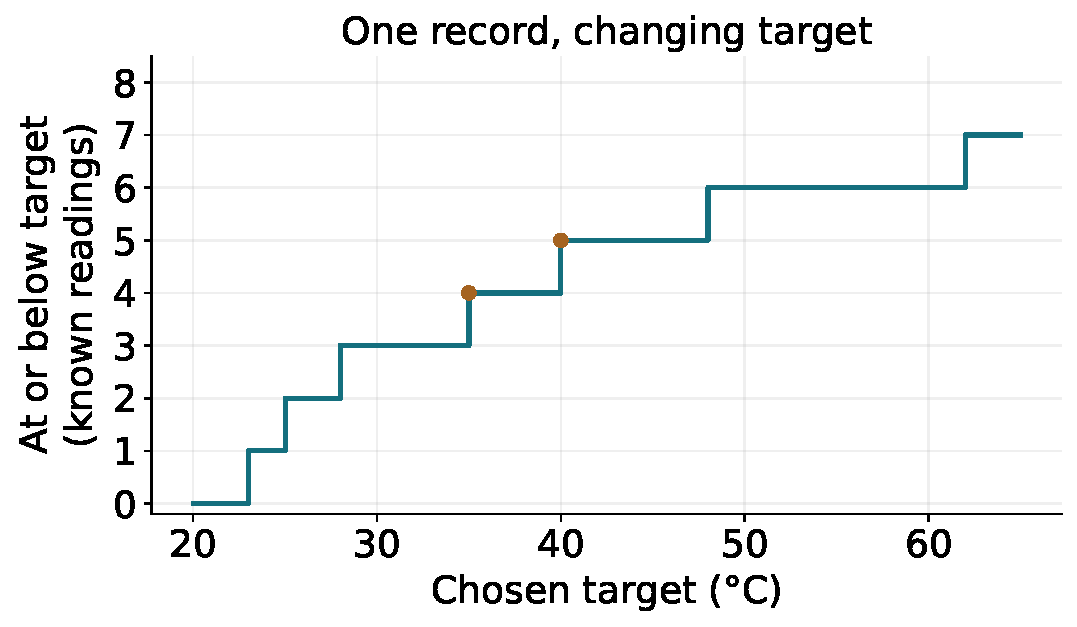
\includegraphics[width=.98\linewidth,height=.69\textheight,keepaspectratio]{presentation-figures/threshold-counts.pdf}\end{frame}
\renewcommand{\notestarget}{notes.pdf\#note-the-first-recorded-qualifying-time}
\begin{frame}[t,fragile,label=slide-recorded-time-and-continuous-crossing]{Recorded time and continuous crossing}
The record contains $T(2)=48$ and $T(3)=40$.
\pause{}
The first qualifying observation occurs at $3$ min. An exact continuous crossing requires a model between observations. With oscillation, even earlier unobserved crossings are possible.
\end{frame}
\renewcommand{\notestarget}{notes.pdf\#note-monotonicity-of-threshold-counts}
\begin{frame}[t,fragile,label=slide-monotonicity-of-threshold-counts]{Monotonicity of threshold counts}
\[
\{i:x_i\leq\theta_1\}\subseteq\{i:x_i\leq\theta_2\}
\quad(\theta_1\leq\theta_2).
\]
\pause{}
Therefore $N_{\leq}(\theta_1)\leq N_{\leq}(\theta_2)$.
\end{frame}
\renewcommand{\notestarget}{notes.pdf\#note-indicators-and-accumulated-counts}
\begin{frame}[t,fragile,label=slide-a-loop-with-paired-observations]{A loop with paired observations}
\begin{verbatim}
for time, value in zip(times, readings):
    category = classify(value, target)
    counts[category] += 1
    if category == "at_or_below" and first is None:
        first = time
\end{verbatim}
Equal list lengths must be checked: \texttt{zip} stops at the shorter input.
\end{frame}
\end{document}
